\documentclass[format=acmtog]{acmart}

\usepackage{blindtext}

\usepackage{graphicx}
\graphicspath{ {./img/} }

\usepackage{subfig}


\usepackage[ruled]{algorithm2e} % For algorithms
\renewcommand{\algorithmcfname}{ALGORITHM}
\SetAlFnt{\small}
\SetAlCapFnt{\small}
\SetAlCapNameFnt{\small}
\SetAlCapHSkip{0pt}
\IncMargin{-\parindent}


%\newcommand{\abs}[1]{\left| {#1} \right|}
%\newcommand{\acos }{ \ensuremath{ \cos^{-1} } }
%\newcommand{\asin }{ \ensuremath{ \sin^{-1} } }
%\newcommand{\atan }{ \ensuremath{ \phantom{\cdot}\text{atan}_2 } }
%\newcommand{\ball}{\ensuremath{ \mathcal{B} }}
%\newcommand{\bigO}{ \ensuremath{ \mathcal{O} }}
%\newcommand{\degree}{\,^{\circ}}
%\renewcommand{\det}[1]{ \ensuremath{ \text{det}\left( #1 \right) } }
%\newcommand{\hull }[1]{ \ensuremath{ \text{convex hull}\left( #1 \right) } }
%\newcommand{\identity}{ \ensuremath{ \mat I }}
%\newcommand{\idx }[1]{ \ensuremath{ \mathbb{#1} } }
%\newcommand{\intersection}{\ensuremath{ \cap }}
%\newcommand{\logand }{ \ensuremath{ \wedge } }
%\newcommand{\logor }{ \ensuremath{ \vee } }
\newcommand{\mat}[1]{\ensuremath{\mathbf{#1} }}
%\newcommand{\interior}[1]{\ensuremath{ {#1}^{\circ} }}
%\newcommand{\boundary}[1]{\ensuremath{ \partial{#1} }}
%\newcommand{\N}{ \mathbb{N} }
\newcommand{\norm}[1]{\parallel {#1} \parallel}
%\newcommand{\proj }[1]{ \ensuremath{ \text{proj}\left( #1 \right) } }
\newcommand{\prox }[2]{ \ensuremath{ \text{prox}_{#1}\left( #2 \right) } }
\renewcommand{\Re}{ \mathbb{R} }
\newcommand{\Z}{ \mathbb{Z} }
\newcommand{\set}[1]{\mathcal{#1}}
\newcommand{\seq}[1]{ \left\{ #1 \right\} }
%\newcommand{\sgn }[1]{ \ensuremath{ \text{sgn}\left( #1 \right) } }
%\newcommand{\smallO}{\ensuremath{ \mathbf{o} }}
\renewcommand{\th}{ \ensuremath{ ^{\text{th}}} }
%\newcommand{\trace }[1]{ \ensuremath{ \text{tr}\left( #1 \right) } }
%\newcommand{\union}{\ensuremath{ \cup }}
\renewcommand{\vec}[1]{ \boldsymbol{#1 } }
\newcommand{\quat}[1]{ \boldsymbol{#1 } }
%\newcommand{\activeset}{ \mathcal{ A } }
%\newcommand{\allset}{ \mathcal{ E } \cup \mathcal{I} }
%\newcommand{\arctantwo}{\ensuremath{\arctan\!2}}
%\newcommand{\crossmat}[1]{\ensuremath{\boldsymbol{#1}^{\times} }}
%\newcommand{\curl}{\operatorname{\text{curl}}}
%\newcommand{\diag}{\operatorname{\text{diag}}}
%\newcommand{\divergence}{\operatorname{\text{div}}}
%\newcommand{\enorm}[1]{\ensuremath{\left\| #1 \right\|_{_2}}}
%\newcommand{\equalityset}{ \mathcal{ E } }
%\newcommand{\feasibledirections}{ \ensuremath{\mathcal{F}} }
%\newcommand{\feasibleregion}{ \ensuremath{\Omega} }
%\newcommand{\func}[1]{{\bf{#1}}}
%\newcommand{\grad}{\operatorname{\nabla}}
%\newcommand{\inequalityset}{ \mathcal{ I } }
%\newcommand{\jacobian}[1]{\ensuremath{\boldsymbol{\mathit{#1}} }}
%\newcommand{\lagrangian}{ \mathcal{ L } }
%\newcommand{\rtm}{$^{\textrm{®}}$} % Registred trademark  \textregistered
%\newcommand{\tangentcone}{ \ensuremath{ \mathcal{ T }_{\Omega} } }
%\newcommand{\vecop}{\operatorname{\text{vec}}}
%\newcommand{\FG}{ \mathcal{G} }
%\newcommand{\FC}{ \mathcal{F} }
%\newcommand{\LS}{ \mathcal{L} }

\newcommand{\model}{ \mathcal{M} }
\newcommand{\modes}{ \mathcal{L} }
\newcommand{\goals}{ \mathcal{G} }
\newcommand{\interpolators}{ \mathcal{I} }
\newcommand{\ipweight}{u}
\newcommand{\dipweight}{\Delta{u}}
\newcommand{\actor}{ \mathcal{A} }
\newcommand{\kine}{ \mathcal{K} }

\newcommand{\mode}{ l }
\newcommand{\interpolator}{ i }

\newcommand{\pos}{ \vec{p} }
\newcommand{\speed}{s}
\newcommand{\ori}{ \quat{\theta} }
\newcommand{\move}{\quat{\theta_m}}
\newcommand{\dtmove}{\dot{\quat{\theta}}_m}
\newcommand{\facing}{{\quat{\theta_f}}}
\newcommand{\dtfacing}{\dot{\quat{\theta}}_f}
\newcommand{\dtpos}{ \dot{\pos} }
\newcommand{\dtori}{ \dot{\ori} }
\newcommand{\blend}{ \vec \omega }
\newcommand{\weight}{ \omega }
\newcommand{\sfunc}{ \textit{Step} }
\newcommand{\interp}{ u }
\newcommand{\dt}{\Delta{t}}

\usepackage{color} 
\definecolor{color1}{rgb}{0.5,0.1,0.1}
\definecolor{color2}{rgb}{0.1,0.5,0.1}
\definecolor{color3}{rgb}{0.1,0.1,0.5}
\definecolor{color4}{rgb}{0.5,0.1,0.5}
\newcommand{\kenny}[1]{{ \color{color1} K: #1}}
\newcommand{\magnus}[1]{{ \color{color2} M: #1}}


\begin{document}
\title{Movement Models for Game Locomotion}


%%
%% The "author" command and its associated commands are used to define
%% the authors and their affiliations.
%% Of note is the shared affiliation of the first two authors, and the
%% "authornote" and "authornotemark" commands
%% used to denote shared contribution to the research.

\author{Magnus Koch}
\email{m.koch@di.ku.dk}
\orcid{1234-5678-9012}

\author{xxx yyyy}
\email{zzzz@wwww.dk}
\orcid{1234-5678-9012}

\author{Fredrik Dalland Holsten}
\email{fredrik@alexandra.dk}
\orcid{0000-0001-6808-4747}

\author{Kenny Erleben}
\email{kenny@di.ku.dk}
\orcid{0000-0001-6808-4747}

\affiliation{%
  \institution{University of Copenhagen}
}

%%
%% By default, the full list of authors will be used in the page
%% headers. Often, this list is too long, and will overlap
%% other information printed in the page headers. This command allows
%% the author to define a more concise list
%% of authors' names for this purpose.
\renewcommand{\shortauthors}{Koch et al.}


\begin{abstract}
%In this paper w
We present a method to extract models from reference animations that can reproduce movement from user input. 
%Although 
Much work has been to done to create realistic full body character animation there is a lack of methods for performing the supplementary task of accurate modeling between user input and future trajectory. This is important for systems that use %\kenny{does reviewer know what this is?} 
weak control signals to guide animation synthesis
%, but e
Especially for computer games where the character position is typically mapped directly to the estimated trajectory with animations overlaid as a secondary effect that is not allowed to diverge. \changed{When a visual discrepancy artifacts appear current practice requires a tedious manual alignment process to avoid this. Our method provides an automated alternative to current practice.} \changed{Input control is ill-defined as the user may not be able to faithfully reconstruct the full movement details using a gamepad. Hence, we regularize the task by introducing control genomes to represent reduced user control signals, thereby deferring complexity to our models.} We further introduce movement models using a modular approach where primitives are combined and we demonstrate a model for plane locomotion in games. Finally the modeling task is further addressed by animation alignment and trajectory estimation where unwanted details are filtered.
\end{abstract}

%%
%% The code below is generated by the tool at http://dl.acm.org/ccs.cfm.
%% Please copy and paste the code instead of the example below.
%%
\begin{CCSXML}
<ccs2012>
   <concept>
       <concept_id>10010147.10010371.10010352.10010238</concept_id>
       <concept_desc>Computing methodologies~Motion capture</concept_desc>
       <concept_significance>500</concept_significance>
       </concept>
   <concept>
       <concept_id>10010147.10010371.10010352.10010380</concept_id>
       <concept_desc>Computing methodologies~Motion processing</concept_desc>
       <concept_significance>500</concept_significance>
       </concept>
   <concept>
       <concept_id>10010147.10010371.10010352.10010378</concept_id>
       <concept_desc>Computing methodologies~Procedural animation</concept_desc>
       <concept_significance>300</concept_significance>
       </concept>
 </ccs2012>
\end{CCSXML}

\ccsdesc[500]{Computing methodologies~Motion capture}
\ccsdesc[500]{Computing methodologies~Motion processing}
\ccsdesc[300]{Computing methodologies~Procedural animation}

%%
%% Keywords. The author(s) should pick words that accurately describe
%% the work being presented. Separate the keywords with commas.
\keywords{Computer Games, Animation Control, Motion Matching}

%% A "teaser" image appears between the author and affiliation
%% information and the body of the document, and typically spans the
%% page.
\begin{teaserfigure}
    \label{fig:teaser:a}
    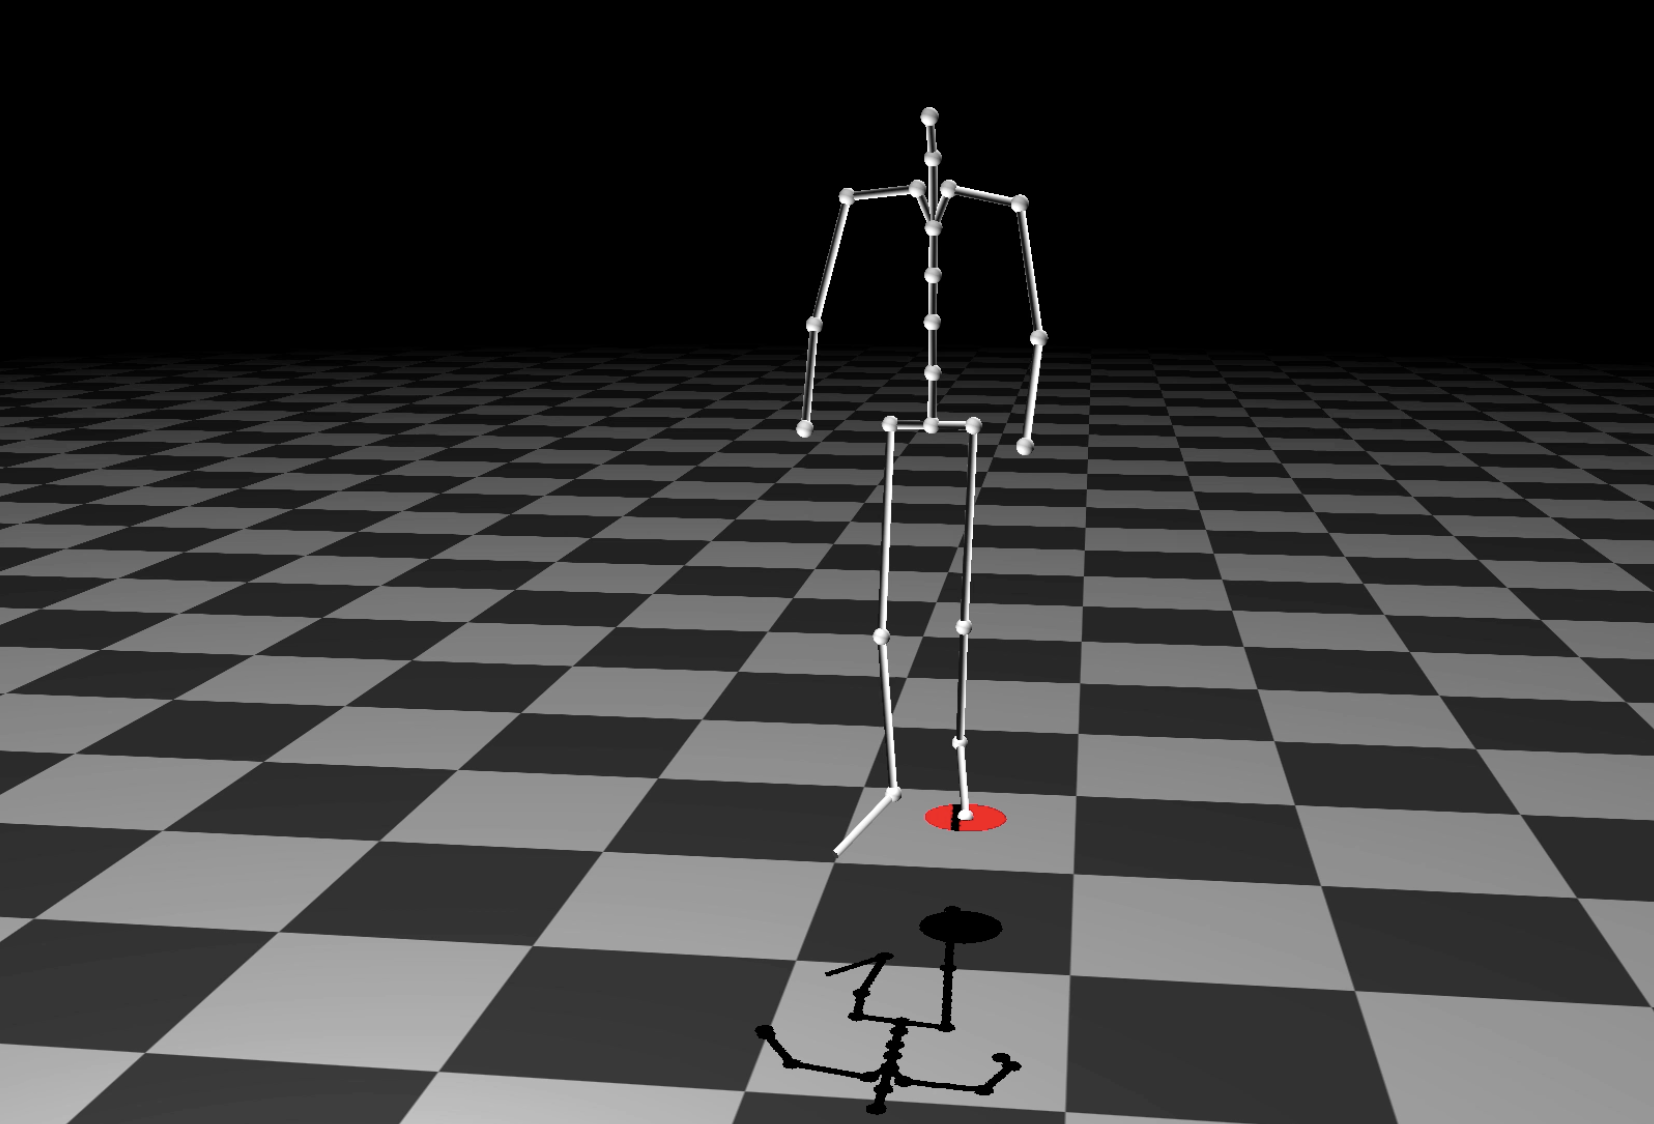
\includegraphics[width=1\textwidth]{img/teaser}
    \protect \caption{
    Our Movement models provide both a weak control signal for interactive games as well as accurate description of the actual motion. The model can be auto-tuned and generated from data offline to generate fluent and consistent motion as seen above.} 
  \Description{Awesome.}
  \label{fig:teaser}
\end{teaserfigure}



\maketitle

% \section{meta}
% \subsection{Method section}
% \begin{itemize}
%     \item Describe animations, annotated control -> genomes.
%     \item Describe model. A what can influence movement ? Velocity. Angular Velocity. Sharpness of desired turn. Style (run etc). Movement templates that react to this, and return updated parameters. Position, and orientation. Rest can be derived.
%     \item Initialize optimization with sane values from physics.
% \end{itemize}

% \subsection{Elevator Pitch A,}
% It is often necessary for developers of interactive applications to understand the coverage (range of motions) available in an animation database or generative animation system. It has been customary to conceptualize coverage as the degree to which a system is able to achieve pre-defined tasks, such as walking from A to B, following a curve etc. We propose an alternative approach where tasks are extracted from the animations themselves in the form of \textit{Control Genomes}, which are parsed by a parametric \textit{Movement Model} to generate movement. The parameters of the Movement Model are fitted for correspondence between the generated movement and the reference animation system. By inspecting the detected Control Genomes and feeding synthetic Control Genomes to the fitted Movement Model, the user is provided a condensed view of the often chaotic details in larger animation sets. This view of coverage is pragmatic as the Movement Model will generally not be able to capture all the variations in the animations. As such we will treat coverage as the identification of stereotypical patterns within the animations.   
% \\\\ 
% We could use a car as example. Currently we would ask, can the car drive from A to B in 5 minutes?. It seems the user pressing the speed continuously. This is our genome. Now we assume that the model is simple acceleration plus wind resistance. We fit the parameters of that model to best describe the movement we have been provided. \\ Previous work should include animation research from the 00s as well as physical simulation / control signal stuff.  
% \subsection{Contributions}
% \begin{itemize}
%     \item Idea to describe coverage through a model that reacts to control genomes.
%     \item Idea to annotate with control signal. Authored fitting
%     \item Description of model for plane locomotion.
%     \item Procedure to fit model under non destructive alterations of animations.
% \end{itemize}
% \subsection{Applications}
% \begin{itemize}
%     \item Analytical tool for animators.
%     \item Displacement of character in computer games. In-place animation played on top.
%     \item Control input to data driven systems such as motion matching or generative neural networks.
% \end{itemize}


% Argument for movement model project: The 'weak control signal' \url{https://www.youtube.com/watch?v=jw0_aBPROGA}, is used to move capsule. So it is important that it fits animations as it provides the root motion.


% \subsection{Elevator Pitch B}
% In game development it is a common construct to have character position driven by a simple algorithmic model that responds to player input.
% \\ 
% In-place animations are then played at the position given by the model at any given time.
% \\
% If the model movement matches poorly with the movement in the animations, the character will appear to float.
% \\
% We propose a general \textit{Movement Model} and optimization framework that ensures synchronization between animations and model. 

% \subsection{Verification}
% Remove root motion from animation. Replay in-place animation on top of movement model. If there is no sliding, we have a perfect match.

\section{Introduction}
Realistic and responsive character animation is important for establishing immersion in computer games. The complexity of human movement makes it difficult to construct such an experience by hand. Instead we record reference data using motion capture and construct animation synthesizers that either stitches clips together, samples inferred statistical models, or learns control policies for a physical model and mimics the animations. Recent advances 
%in both industry and research communities 
show a strong tendency towards complex closed systems guided by weak control signals. Notably \citep{holden.ea20} and \citep{Bergamin19} uses a spring-damper system due to \citep{kermse.04} for a motion matching system, while \citep{startke20} generate control trajectories by upsampling an unspecified smooth user input using a neural network. In \citep{zhang18} an interpolation between current and desired direction is fed directly to a generative model and in \citep{peng17} a physical model is trained to follow randomly generated paths by allowing a 2 meter divergence. \kenny{Our work use XXX? or is similar to YYY? or ?}

To our best knowledge it has not been investigated how to construct and synchronize weak control signals to animation synthesizers for full body locomotion. This is important for computer games. It is an industry standard in AAA productions to have a gameplay layer that controls changes to character position and a separate animation layer that tries to generate animations that matches the changes in positions \citep{holden18}. We suggest the term \textit{movement model} to describe the gameplay layer logic that controls character position in response to player input. In game productions the movement model is carefully tuned by designers to give a response that \textit{feels appealing}, it is used to predict future character movement and even for analyzing the validity of game levels. These industry practices poses requirements to how we construct our movement models. 

The movement model seems an ideal control signal for animation synthesizers. We have a history of movement available and can integrate the model for predictions.Hence, the movement model is both a weak signal and describes the actual movement of game characters and this introduce a challenge. If there is a disconnect between the movement model and the animation synthesizer output, we might allow the animations to diverge from the movement model and later catch up. But this severely impacts the types of game experiences that can be created as we loose exact positioning of our character and it changes the feeling of movement in response to player input which is critical for immersion \magnus{(REF)}. If we enforce synchronization between the two layers artifacts such as foot sliding and a general degradation of realism and quality kick in. It is an industry standard to carefully synchronize animations and movement models by hand at great economical cost to avoid these issues. \changed{We show how current best practice compared to our method in Figure \ref{fig:teaser}.}

%We propose that it is a valuable effort to investigate movement models and suggest a procedure to do so. It is a task that runs parallel to the more researched area of modeling full body kinematics, and has stricter requirements for simplicity as models should be extremely fast to evaluate and open for manual tweaks to get the feeling of movement just right. 
We propose to investigate movement models as a valuable mechanism for handling both weak control and actual motion description. In order to be applicable in AAA game production the models are required to be simple, as automated as possible to avoid unnecessary manual labour, extremely fast to evaluate, and open for manual artistic tweaks to change the feeling of movement if needed.

In the following pages we introduce a method for composing movement models from primitives that can be automatically fitted to reference animations using auto differentiation. We suggest a model composition for plane locomotion and show procedures to simplify and align the animations to avoid modeling complex and unnecessary details while preserving visual quality. Our modeling task is ill-posed since in the limit player input could contain complex low level control signals similar to what is found in the animations, which would greatly reduce requirements to the model as the control signal would itself represent what we are trying to model. We regularize the task by using the novel concept of \textit{control genomes} to formalize the reduction of low level control input to high level signals corresponding better to expected player behavior. Finally we present a procedure to determine movement in animations from foot contact analysis which was discovered as a side effect of our work and can be used in its own right.


\section{Related work}
The complexity of human movement is evident in character animation research where general solutions are rare and it is often necessary to develop tailor made solutions for different types of tasks. Our work relates most directly to path following task as in \citep{lee10}, \citep{holden.16} where a detailed movement is specified by the user and tracked by the animation synthesizer. Our approach is in principle generally applicable, but we restrict ourselves to path following. In these systems we often find analogies to movement models whenever high level user input from mouse or gamepad is projected into task specifications such as a series of game coordinates to specify a path. There is a necessary tradeoff between the quality of the synthesizer animation and the accuracy of the tracking which is often exposed as an adjustable parameter.

\subsection{User input smoothing}
Counterparts to our movement model concept are found in both industry and research settings whenever a user input is translated to a path that is either tracked by an animation synthesizer or used to explicitly position the character.

For the industry setting the division between gameplay and animation layers described by \citep{holden18} is reflected in state of the art tools such as Unreal Engine and Unity. Both expose animation systems with the ability to toggle root motion for animation clips. In our experience root motion is primarily used for static content such as cinematics. In interactive gameplay characters move using ad hoc systems analogous to the movement model with in-place animations played on top. Character movement is controlled by transitioning towards the direction supplied by the user using an assortment of smoothing techniques such as lerp, exponential decay or damped springs as seen in \citep{buttner20} and \citep{holden21}.

In research a similar approach is often found as in \citep{mccann07}, \citep{holden.16}, \citep{Zhang18} and \citep{startke20}. The latter augments a smoothed user input by projection to a lower level control space similar to trajectories found in the reference animations, which illustrates the discrepancy between the weak control signal and the synthesize motion common to these methods. A compromise is struck by either allowing the synthesized motion to diverge from the control signal or accepting visual artifacts.

A variant of this approach is found in \citep{treuille07} where an offline system tracks a path drawn by the user. In this case we have no movement model as the user input is exactly the low level control signal. Oppositely \citep{kovar02} use reward functions to provide less constrained control when the user specifies goals such has 'end position' that have no path requirements, and in \citep{lee18} 'straightness' and other stylistic traits contribute to similar rewards. In these cases the movement model is embedded in the animation synthesizes, but could be separated by augmenting the reward functions. Since high level tasks are used to allow the synthesizer some freedom, the specification is most often kept simple. A hybrid approach in \citep{lee10} track a control direction from the user with no explicit path but with a short horizon tending toward a path specification.

\subsection{Motion planning and control theory}
Convert high level task specification into low level control that makes system (robot (motion planning) or system of differential equations (control theory)) perform task.
Here we have an unknown system and would like to figure out the control signal. Inverse problem of ours. We have the low level control signal and want to figure out a system that can reproduce that. High level task are users overal intention, move though city.

\subsection{Animation coverage}
Movement model is like a model to represent the coverage of the animation system, in a format that is simpler than the animations themselves. Ectract trajectories from animation (Buttner), train model to convert (Local phase thing). 

\subsection{Function approximation}

Dynamic movement models \ref{https://studywolf.wordpress.com/2013/11/16/dynamic-movement-primitives-part-1-the-basics/} have a pd control with another funciton to mimic robots actual behaviour. We move some of this into a model that is simple and can be inspected, and some of the complexity is handled by trajectory alignment and analysis. "Point attractor dynamics plus overlay with complex function".

\subsection{Motion matching and animation graphs}
Classical graph based animation systems such as \citep{treuille07} have users draw directories as control signal for path following task. Here the mapping from abstract control space, ie. 'turn right', to a motion plan is entirely up to the user. This bypasses the need for a movement model, at the cost of reduced quality when the users requests paths that are not present in the animation data.



Generatetive neural networks Weak Control Signals
    Starke use weak signal and input noise. More noise, better animation, and less control.

    \citep{lee18} supplies a distant control target target such as a final position, and combined with a attributes such as 'straight' to guide the movement.

Graph based approach 
    Hodgins, motion fragments

Control Theory

Function approximations 
    RBF, movement primitives

Motion planning
    Robotics (deep loco good to look at)
    Graph based stuff

\kenny{what is state of the art work to compare against?}


\subsection{Animation Warping}
Animation warping can be viewed as a generative model trained on $D$. 


\section{Optimal Control Genome Method}
Human movement is a complex interplay between intentions within the brain and the physical environment. The thought to 'walk-forward' triggers and array of intractable optimization  

In the following we will introduce a method for optimal synchronization between a Movement Model and a set of animations given our Control Genomes. There are 4 main parts to the method. 
\begin{itemize}
    \item \textbf{Control Genomes} extracted from animations.
    \item \textbf{Movement Model} that generates a movement given Control Genomes.
    \item \textbf{Animation Alignment} and filtering. 
    \item \textbf{Optimization procedure} that fits exposed parameters of all the above systems to minimize the difference between the Movement Model- and animation trajectories.
\end{itemize}
Figure \ref{fig:movement:model} illustrates the definitions and concepts of a movement model.
\begin{figure}
    \centering
    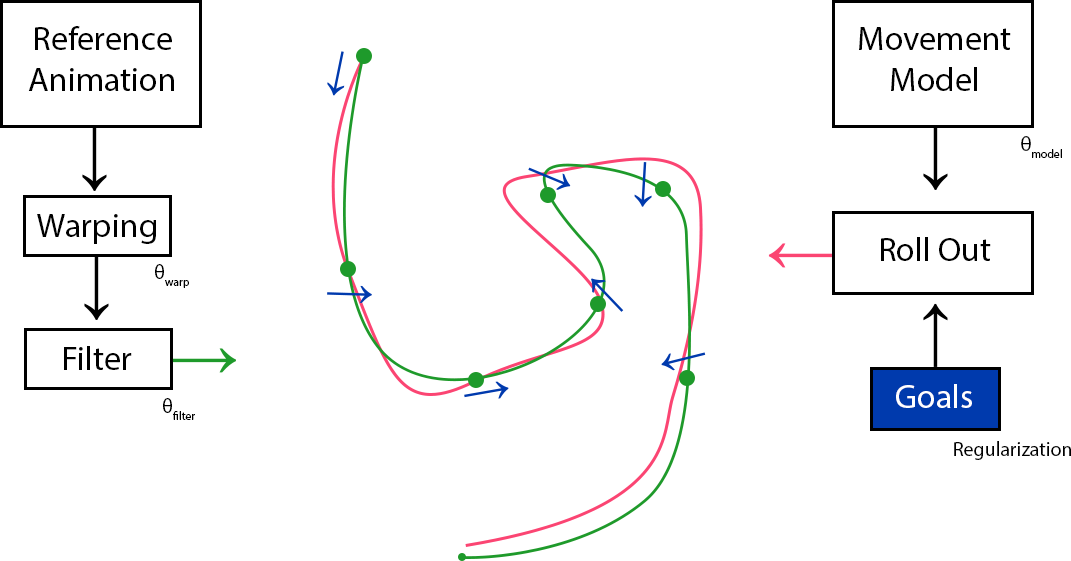
\includegraphics[width=0.75\linewidth]{img/method-overview.png}
    \caption{Theta values indicate parameters subject to optimization. Goals are fixed to add regularization}.
    \label{fig:movement:model}
\end{figure}

\subsection{Control Genomes}
We define Control Genomes as signals that can generate movement. They are a combination of intentions and enough contextual state to follow the Markov principle. As an example a position, direction and time is a control genome for a straight walk. Conversely a straight walk contains a latent control genome (position, direction, time). Under this naive framework we quickly realize that multiple straight walks could be associated with a single control genome. We further impose the constraint that control genomes must disambiguate movement. That means a unique control genome maps to a unique movement. In our simple example we might resolve conflicts by adding a style parameter and assign values such as 'brisk walk' or 'dragging feet' to our control genomes. 

Control genomes can have a direct counter part in the host application such as user input through a game controller or navigational path from an AI system, and therefore can also be viewed as tasks that are carried out by the animations, for instance turn right. In general we want the control genomes to be of minimal size, since in the limit we could have the animation itself as the control genome. We say that a genome is in \textit{reduced} and \textit{segmented} form if it contains no repetitions and removal of information would break either the Markov property of the disambiguation constraint. 

\begin{figure}
    \centering
    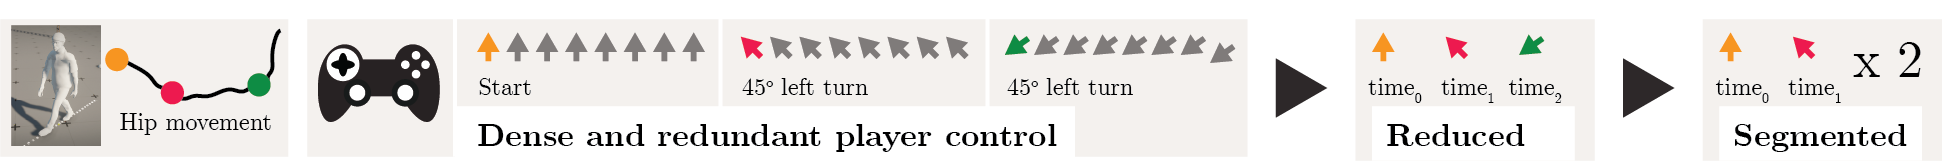
\includegraphics[width=1\columnwidth]{img/controlgenome.png}
    \caption{Control Genome.}
    \label{fig:control:genome}
\end{figure}

Figure \ref{fig:control:genome} shows an example where an animation has been assigned a control genome. Each frame is annotated with a 2D-control direction corresponding to stick input from a game controller. A dense and redundant control genome contains the entire skeletal animation as well as the annotated directions. The animation has two similar right turns so we get a single segmented control genome by splitting the redundant genome in two identical parts. We then trim all unnecessary information from the genome to get the reduced form which only contain a starting position and two direction offset in time. This last step assumes that we are capable of regenerating the animation from the reduced genome using a model we will refer to as a \textit{Movement Model}. A [Control Genome, Movement Model]-pair describes an animation exactly when the Movement Model can regenerate the Animation from the Control Genome.  In practice it is not possible to develop accurate generative or predictive models for human movement. So we will allow our animations to undergo non destructive transformation such as smoothing and path adjustment, and only expect our model to regenerate a fraction of the complete signal, such as the trajectory. 

We will now proceed to a formalized description of control genomes. The input to our method is an annotated animation. Let $\anim^{\dimas,\dimaa}_\dimat$ denote $\dimat$ frames of animation of a skeleton with $\dimas$ degrees of freedom, where each frame is given an $\dimaa$-dimensional annotation. 

We assume there exist a automated or manual Retrieve-and-Collapse function, $\reco$,  that extracts all reduced and segmented control genomes present in the animation and for each maintains a pairing to all $k$ corresponding un-annotated segments of the source animation. That is $\reco$ converts a source animation into an associate map, $\lut$, that uses genomes as keys and un-annotated segments of source animation as values. We may write $\reco(\anim^{\dimas,\dimaa}_\dimat) \rightarrow \lut$. Now given the $i\th$ control genome of dimension $\dimg$ we have
\begin{equation}
 \lut(\genome^g_i) \rightarrow \left\{\anim^{\dimas,0}_{\dimae_0},\ldots,\anim^{\dimas,0}_{\dimae_k}\right\}   \,,
\end{equation}
where $\dimae\ll\dimat$ refers to a segment of the full animation and $k$ is the number of segments matched to the $i\th$ control genome.

We define two parametric projections, $\model$ and $\edit$, to a shared $\dimes$-dimensional space, $\mathcal{R}^{\dimes}$, as follows
\begin{align}
\model(\paramm,\genome_i^{\dimg}) 
&\rightarrow 
\mathcal{R}^{\dimes}    \,,
\\
\edit(\parame,\anim_{\dimae}^{\dimas,0})
&\rightarrow
\mathcal{R}^{\dimes} \,,
\end{align}
where $\paramm$ and $\parame$ are free parameters to be optimized for later. We call $\mathcal{R}^{\dimes}$ an evaluation space and it will usually have a natural counterpart in the application such as the trajectory (position and orientation of character over time).

Intuitively $\model$ is a Movement Model capable of generating movement or more accurately an evaluation space representation from the control genomes. $\edit$ corresponds to the adjustment we allow our animations to undergo, such a smoothing or more advanced manipulation. The optimal parameters for a single control genome are found as the minimization of the L2-norm.
\begin{subequations}
\begin{align}
    \gnorm(\paramm,\parame,\genome_i)
    &\equiv
    \sum_{\anim_k\in\lut(\genome_i)}
    {
        \frac{1}{2}
        |\model(\paramm,\genome_i)
        -
        \edit(\parame\anim_k)|^2
    }
    \label{eq:optim:single}
    \\
    \paramm^*,\parame^*
    &\equiv \arg\min_{\paramm,\parame}
    {
        \gnorm(\paramm,\parame,\genome_i)
    }
\end{align}
\end{subequations}
When we want constant parameters across the fitting of multiple control genomes an additional term is added to the minimization. 
\begin{equation}
    \vec{\paramm^*},\vec{\parame^*}
    \equiv 
    \arg\min_{\paramm,\parame}
    \left(
        \sum_{\genome_i}
        \gnorm(\paramm^i,\parame^i,\genome_i)
    \right)
    +
    VAR(\vec{\paramm},\vec{\parame})
\end{equation}
Where $\vec{\paramm^*},\vec{\parame^*}$ is the full set of parameters and $\paramm^i,\parame^i$ are the parameters fitted to $\genome_i$.

\subsection{Movement Model}
In this section we will describe how movement can be generated from control genomes using a Movement Model. We will examine plane locomotion and limit the output of the model to trajectories that is a time series of connected positions and facing directions. 
Conceptually there are no limitations on the complexity of the models we chose. Dense neural networks [ref] or muscle based physical simulations [ref] are capable of even generating full body locomotion. However we would like a model that exposes easily and exactly tweakable parameters to the game designers and animators. In many game scenarios micro timings and the 'feel' of the character movement are core parts of the user experience. Accordingly we need descriptive models, that can still be transparently manipulated by the artists. 

As described in the previous section a control genome consists of an initial state paired with a sequence of control inputs. Let $\pos_{t=0},\facing_{t=0}$ describe the initial position and facing angle of the character. Player input is supplied through standard gamepad control using stick direction and button presses with $\controlface_t, \controlmove_t$ representing the desired facing and movement directions at time $t$. Further parameters can be added to support different movement styles.   

A sequence of movement is generated by recursive updates to the genome state by the movement model.
%\begin{subequations}
\begin{align}
    \pos_{t+\dt},\facing_{t+\dt}&\leftarrow[\pos,\facing,\controlface,\controlmove]_t,\dt\label{eq:move:update}
\end{align}
%\end{subequations}
The update  acts as motion planning by controlling how the current state gradually transitions towards a new state as defined by the Control Genome. We impose a restraint to model this transition process according to the characteristics of the reference animation, by inserting recursive calls to update function as $\model$ in the objective function (\ref{eq:optim:single}).

We construct the planning function in \ref{eq:move:update} as a composition of planning primitives. Each primitive exposes a set of adjustable parameters and performs input to output mapping using various interpolation methods. In the limit the compositions could approximate full neural networks, but should be kept simple enough for human manipulation of each parameter while maintaining the capability to model the movement in the reference animations.     

Fig [??] illustrates the 3 planning primitives we use to model plane locomotion. A Critically damped spring $out\leftarrow{}\spring{(in,t,k)}$ exposes a spring coefficient $k$ used to control the drag of the input variable towards the target $t$. The 1D-Map $out\leftarrow{}\mapo(in,k)$ uses spline interpolation over knots in $k$ to map a parametric input to a line position. The 2D-map $out\leftarrow{}\mapt([in_x, in_y], k)$ uses barycentric coordinates to interpolate polygon knots in $k$ according to a 2 dimensional grid position given as input.    

As an example we propose a Movement Model for plane locomotion typical for 3rd person computer games that strikes a compromise between simplicity and expressiveness. We use the convention that i refers to intermediary values during the model update. First the position and facing information contained in the Control Genome state is augmented with derived values $\speed, \move, \angularspeed$ for speed, move direction and angular speed ie. rate of change of the movement direction. We also compute $\diffmove=||\statemove-\controlmove||$ as the absolute error between the state and control values for movement direction. A Movement model is constructed by first describing changes related to speed.

\begin{subequations}
\begin{align}
    \speed_{t+\dt}&\leftarrow{}\spring(\speed_t,\speed^\intermediary,k^\intermediary)\\
    \speed_\intermediary&\leftarrow{}\mapt([\angularspeed_t,\diffmove],\param_0)\\
    k_\intermediary&\leftarrow{}\mapo(\speed_t-\speed_i, \param_1)
\end{align}
\end{subequations}
Here $\param_1$ models the acceleration of the model depending on the relative change in speed, and $\param_0$ models planning of the target speed depending on the current angular speed and the required change to movement direction.

Modeling of changes to movement and facing directions are added.
\begin{subequations}
\begin{align}
    \move_\intermediary&\leftarrow\spring(\move_t,\controlmove_t,\mapt([\speed_{t+\dt},\diffmove], \param_2))\\ 
    \pos_{t+\dt}&\leftarrow{}\pos_t+\speed_{t+\dt}{}rotate(forward,\move_\intermediary)\\
    \facing_{t+\dt}&\leftarrow\spring(\facing_t,\controlface_t,\mapt([\speed_{t+\dt},\difffacing], \param_3))
\end{align}
\end{subequations}
Here $\param_2$ and $\param_3$ model planning of movement and facing direction dependent on the current speed and facing values and the differences to the control targets.

If we use 9 knots for the 2D blends, and 4 four the 1d, we have a total of 4 + 3*9 tuneable parameters. An example plot of the model using reasonable parameters is depicted in fig ??.

An analytical model like this can be of great practical use to the game developers. The parameters have direct links to relatable properties in the animation which makes it easier to tweak the behavior of the model. On the other hand, the analytical approach requires that the designers are able to adequately model the complexity of the movement. When this is not the case, we can apply machine learning techniques to discover latent properties of our animation set. 

One approach is to extract a limited latent variable set using a dense neural network and then feed the latent variables to a set a primitives which are weighted to give the final output. 
Alternatively, we could apply a hybrid approach by discovering correlations in the data by automated statistical analysis, but still allow the designer to setup the primitives and chose which parameters should be used. 

Finally we note that multiple local Movement Models can be easily combined. Transitions between models can be established using the same primitives. In practice it is often sufficient to use a single 1D blend. For instance the shift between 'run' and 'walk', which could require individual models, is usually distinct and of limited complexity and duration. 

\subsection{Motion Alignment and Filtering}
It is difficult to capture consistent animation data. Treadmills can be used to maintain constant speeds, but this poses a limitation in maneuverability. It requires accurate high frequency control to reproduce the subtle changes in speed and direction that are present even if the subjects are directed to move in a consistent manner. It is often possible to apply minor changes to the speed and direction of the recorded animation, without loss of visual quality. By allowing this, we can align an animation set with respect to speed and movement patterns. 

An adjustment curve contains pr. frame changes to rotation and speed of an animation, and is applied as modifications to the root joint of the animation. An adjustment curve containing all zeros and a single $\frac{\pi}{2}$ would for instance modify a straight walk to have a 90 degree turn over a single frame. To maintain a smooth and subtle modification we can interpolate sparsely distributed key frames and impose limitation on the amount of adjustment allowed pr. frame. We found that various heuristics such as scaling the adjustment depending the relative amount of movement at a given frame, or by the distance from a frame the to nearest control genome, helps maintain the quality of the animation (se fig for reference). Post processing techniques such as foot-IK, Paragon step length increase, or pivoting rotation around foot contacts can also be applied.

Even perfectly consistent animation data contains hard to model fluctuations due to the way humans move. [ref] illustrates the difficulty of deriving a stable position from animation data. We apply a modulating kernel based filter similar to [ref] before the application of the adjustment curve. We use $Adjust(\theta_a,Filter(\theta_f\anim^{\dimas,0}_\dimat))\rightarrow{}[\pos_0,\facing_0, \ldots \pos_t\facing_t]$ as $\edit$ in the objective function (\ref{eq:optim:single}) where $\theta_a, \theta_f$ represent the adjustment curve values and filter kernel weights respectively.

\subsection{Optimization}
When the Movement Genome, Movement Model and the alignment and filtering procedures have been defined, we face an optimization problem consisting of 100s of parameters and many local minima. Fig ?? illustrates how the parameters are distributed across the full system. \magnus{Missing: Genomes can be slightly modified. Changes are in $\theta_G$ which needs to be defined}.

The dimensionality of the parameter space makes it infeasible to use straight forward techniques such as finite differences. We attack the problem by using auto differentiation with PyTorch for the optimization procedure. Having the gradients available we can use line search techniques such as Gradient Descent or Stochastic Gradient Descent which is available in PyTorch.

To use a global learning rate, we normalize the range of all parameters and apply fixed constant scaling. This is easily doable since most parameters have direct physical counter parts such as velocity, turn angles etc. Scale values can then be identified by doing a pre-pass over the animation. This in turn limits the impact of local minima, as the optimization can be given plausible initialization values.

L1 and L2 regularization is applied to most parameters to avoid 'oscillating' interpolations between extreme knot values which can be difficult to interpret and modify for a human. Similar regularization is applied to $\theta_a$ and $\theta_G$ where large values implies divergence from the ground truth present in the Genomes and reference animation.

Auto differentiation requires continuity across the parameters space, and some care must be taken to achieve this. Specifically we ensure that our primitive function are continuous and use leaky relu outside valid ranges to support correct derivates here. 

\section{Experiments}
A series of animations was recorded using the inertial sensor based XSens suit and a single human subject. The raw sensor data was cleaned using the automatic post processing procedure available in the XSens MVN Animate Pro software application.
The movement set was inspired by the structure of locomotion sets used in game production. The subject was instructed to keep the movement consistent and to follow the various movements closely.   

\subsection{Movement Characteristics}
\subsubsection{Purpose}
Illustrate the problem we wish to solve using 1-2 video examples.
\subsubsection{Content}
Show that basic animations have complex root motions that are difficult to replicate using standard 'weak control signal' (splines, springs). 
Show that trivial approaches (smoothing) does not solve problem in convincing way.
\paragraph{Videos}
\begin{itemize}
    \item Show character moving straight and in curves. Trace complex root motion. Highlight the presence of both high and low frequency information in the plot.
    \item Show character running straight with smoothed trajectory. Highlight problems. Show turning characters and illustrate how superficially 'identical' turns are actually very different.
\end{itemize}
\paragraph{Figures}
\begin{itemize}
    \item Plots of trajectory and weak control signal paths.
    \item Plots of smoothing effects
\end{itemize}

\subsubsection{Draft}
Final text

\subsection{Fitting Movement Model}
\subsubsection{Purpose} Show that we are able to solve problem using 3-5 video examples (didactic).
Show how various models can be fitted to data (that has itself been adjusted). 
\begin{itemize}
    \item Straight movement. Walk and run. 
    \item Multiple straight movements. Walk and run. 
    \item 180.
    \item Multiple 180s.
    \item Banking
    \item Multiple banking
    \item 45 turn
    \item Multiple 45 turn
    \item 90 turn
    \item Multiple 90 turn
    \item Mixed modes
\end{itemize}
Additionally we could look at animations published by ubisoft.\url{https://github.com/ubisoft/Ubisoft-LaForge-Animation-Dataset}

\subsection{Application}
\subsubsection{Purpose} Show that our solution has interesting applications using 3-5 video examples (eye candy).
Replace standard control signal with our model.
\begin{itemize}
    \item{Replay animations to illustrate correct root motion}
    \item{Use with motion matching} exponential decay = uttner, Holden Spring damper Kermse 2004].
    \item{use generative neural network} Can we avoid floating character ?
\end{itemize}


\section{Discussion and Limitations}
We have presented a method to 

We have demonstrzte thjat our model can fit to local segment, but a global fitting remains as a challenge.

heterogenous animation. Actor can choose to turn more abrubtly. We can fix some witha lignment, but this makes movementm unnatural. We can add more to conotrl genome but this conflicts with standard game pads and user capabilities. we can then use of method as a filter insted. Given a large database we filter stuff that is too different.


We would like to extend our concept of control genomes. Can they be formalized even more ? Could we develop a set of heuristics to extract from animations in a more structured manner ? 
We would like to investigate more primitive types. Further compare how different primitives can be used for various types of locomotion.

More diverse animation tests.

\section{Conclusion}
We have presented a method for designing character controllers in computer games that react to user input and generate movement similar to reference animations. Since user control is not inherently restricted we use control genomes to ensure that complexity is either contained in movement models or entirely removed by animation alignment. We suggested a movement model for plane locomotion and applied our method to a set of dance card animations similar to those found in industry productions to demonstrate that auto differentiation can be used both for alignment and parameter estimation.  




 \appendix
 
 \section{What you need to know?}
\blindtext

  %%
%% The acknowledgments section is defined using the "acks" environment
%% (and NOT an unnumbered section). This ensures the proper
%% identification of the section in the article metadata, and the
%% consistent spelling of the heading.
\begin{acks}
bla blah
\end{acks}


\bibliography{movement-model-for-motion-matching}{}

\end{document}

